
\documentclass[prd,amsmath,amssymb,floatfix,superscriptaddress,nofootinbib]{revtex4-1}
\usepackage{bm}
\usepackage{amsmath}
\usepackage{epsfig}
\usepackage{color}
\usepackage{natbib}
\usepackage{textcase}
\usepackage{graphicx}
\usepackage{ifthen}
\usepackage{xstring}
\usepackage{graphicx}
\usepackage[utf8]{inputenc} 
\usepackage{amssymb}
\usepackage{latexsym}
\usepackage{epstopdf}
\epstopdfsetup{update}
\DeclareGraphicsExtensions{.ps, .png}
\epstopdfDeclareGraphicsRule{.ps}{pdf}{.pdf}{ps2pdf -dEPSCrop -dNOSAFER #1 \OutputFile} 
\usepackage{dcolumn} 
\usepackage{multirow}
\usepackage{appendix}
\usepackage{footnote}
\usepackage{tabularx,ragged2e,booktabs}
\usepackage[normalem]{ulem}
\usepackage{float}
\restylefloat{table}

\newcommand{\tauhi}{$\tau_{\rm hi}\,$}
\newcommand{\taulo}{$\tau_{\rm lo}\,$}

\newcommand{\refsec}[1]{section~\ref{sec:#1}}
\newcommand{\refeq}[1]{Eq.~(\ref{eq:#1})}
\newcommand{\refssec}[1]{section~\ref{subsec:#1}}
\newcommand{\reffig}[1]{Fig.~\ref{fig:#1}}
\newcommand{\refFig}[1]{Fig.~\ref{fig:#1}}
\newcommand{\curv}{{\cal R}}
\newcommand{\xef}{x_e^{\rm fid}}
\newcommand{\xmax}{x_e^{\rm max}}
\newcommand{\zmax}{z_{\rm max}}
\newcommand{\zmin}{z_{\rm min}}
\newcommand{\xemin}{x_e^{\rm min}}

\newcommand{\ra}{\rightarrow}
\def\max{_{\mathrm{max}}}
\def\lsim{\mathrel{\raise.3ex\hbox{$$<$$\kern-.75em\lower1ex\hbox{$\sim$}}}}
\def\gsim{\mathrel{\raise.3ex\hbox{$$>$$\kern-.75em\lower1ex\hbox{$\sim$}}}}

\newcommand{\beq}{\begin{equation}}
\newcommand{\eeq}{\end{equation}}

\newcommand{\bea}{\begin{eqnarray}}
\newcommand{\eea}{\end{eqnarray}}

\newcommand{\wh}[1]{\textcolor{blue}{#1}}
\newcommand{\ch}[1]{\textcolor{red}{#1}}

\def\mnras{Mon.\ Not.\ R.\ Astron.\ Soc.\ }
\definecolor{darkgreen}{cmyk}{0.85,0.2,1.00,0.2} 
\definecolor{purple}{cmyk}{0.5,1.0,0,0} 
\def\physrep{Phys.~Rep.}

\definecolor{ultramarine}{rgb}{0.07, 0.04, 0.56}
\definecolor{cadmiumgreen}{rgb}{0.0, 0.42, 0.24}
\definecolor{indigo(dye)}{rgb}{0.0, 0.25, 0.42}
\usepackage[linktocpage=true]{hyperref}
\hypersetup{
colorlinks=true,
citecolor=ultramarine,
linkcolor=cadmiumgreen,
urlcolor=indigo(dye),
pdfauthor={},
pdftitle={},
pdfsubject={}
}


\begin{document}
	
\title{Reionization Planck 2018 \\
Notes during paper writing phase}

\author{Chen Heinrich}
\author{Wayne Hu}
 
\maketitle

\section{Comparison to previous results}

The Planck collaboration has released constraints on the total optical depth $\tau$ with a steplike model parameterized by the tanh function, which has evolved from $\tau = 0.067 \pm 0.022$ (Planck 2015) to $\tau = 0.055 \pm 0.009$ (Planck 2016), then to $\tau = 0.0506 \pm 0.0086$ (Planck 2018) \todo{[cite papers]}. The major improvement comes from clean-up of systematics in the High Frequency Instrument (HFI) data. 

In Planck 2018 VI, using only \texttt{SimAll} data and fixing all cosmological parameters including $A_s e^{-2\tau}$, the optical depth constraints was found to be $\tau = 0.0519^{+0.0030}_{-0.0079}$ for the tanh model, 
$\tau = 0.0504^{+0.0050}_{-0.0079}$ 
for the FlexKnot method (with flat $\tau$ prior) and 
$\tau = 0.0487^{+0.0038}_{-0.0081}$
for the PC method but using the prior inversion procedure
discussed \S\ref{sec:note_on_priors} and attributed to the slightly lower central value from the PC method to the fact that the priors contain unphysical models. [do we want to check whether the prior inversion procedure could cause a shift at this level? do we want to evaluate this statement?]

They also found the upper limit on high-redshift optical depth to be: $\tau(15, 30) < 0.006$ for the FlexKnot method with a flat $\tau(15, 30)$ prior or $<0.007$ with a flat knot prior. The PC result for the upper limit was not computed. 

Compared to our PC results ($\tau(15, \zmax)_{\rm PC,\, \zmax=30} < 0.023 \; (95\% \mathrm{CL})$), the FlexKnot upper limits are too stringent. The difference is not attributed to the inclusion of unphysical models due to the truncation at 5 PCs as we showed in \S\ref{sec:example2} with a concrete example of the two-step model. We showed that for this chosen physical model, the $\tau(15, 30)$ upper limits derived from the full Planck likelihood without using any PCs were already not compatible with the FlexKnot upper limits, while the PC results were compatible. So the discrepancy cannot be attributed to the prior choice in the PC results. It also seems that the inclusion of unphysical model would in any case shift the optical depth at high-redshift toward more negative values, which would decrease rather than increase the upper limit. 

[just noticed that our tau(15, 30) $<$ 0.023 result is with srollv2, and flexknot tau(15,30) $<$ 0.007 is with \texttt{SimAll} likelihood. In our analysis \texttt{SimAll} to sroll2 had a 0.004 increase in total tau. I should run the tau(15, 30) constraint on the \texttt{SimAll} chain as well just to double check.]

[Need to address Planck2018 cosmology paper claim: ``The PCA result is slightly lower, and is partly affected by the imperfect physicality priors that allow unphysical negative ionization fractions."]

[Also, they only used \texttt{SimAll} likelihood, fixed all other cosmological parameters (including $A_s e^{-2\tau}$). Wondering if that does anything to the difference between our results]

%%%%%%%%%%%%%%%%%%%%%%%%%%%%%%%%%%%%%%%%%%%%

\section{Some Numbers}

\textbf{Planck official results 2015, 2016, 2018} \\

\begin{itemize}
    
    \item Planck 2015 results (LFI): $\tau = 0.067 \pm 0.022$ (68\%) \\

    \item Planck 2016  intermediate results (LFI): $\tau = 0.055 \pm 0.009$ (68\%) \\
    
    \item Planck 2018 results: $\tau = 0.0506 \pm 0.0086$ (68\%) \\

\end{itemize}

\textbf{Planck 2018 paper} \\

Here lowE means lowE data only, fixing all other cosmological parameters including $A_s e^{-2\tau}$\\

\begin{itemize}

\item $\tau = 0.0519+0.0030-0.0079$ (lowE; flat $\tau$ prior; TANH)(68\%); \\

\item $\tau = 0.0504+0.0050
-0.0079$ (lowE; flat $\tau$ prior; FlexKnot)(68\%); \\

\item $\tau = 0.0487+0.0038
-0.0081$ (lowE; flat $\tau$ prior; PCA)(68\%).

\end{itemize}

\textbf{Upper limit on high-redshift optical depth} (only given for the FlexKnot method):

$\tau(15, 30) < 0.006$ (lowE, flat $\tau(15, 30)$, FlexKnot); \\

$\tau(15, 30) < 0.007$ (lowE, flat knot, FlexKnot).\\

Statements to address:

\begin{enumerate}
    \item {\textbf{Statement on prior in Planck 2018}:  ``Heinrich \& Hu (2018) construct a prior that is uniform on $\tau$, but which increases the allowed unphysical parameter space and is chosen a posteriori. Here we instead use the flat prior constructed by the procedure described in Millea \& Bouchet (2018) and Handley \& Millea (2019), which does not admit extra unphysical models and gives the most generic prior that leaves the prior on $\tau$ uniform."}
    
    \item {Is this statement on tanh in Planck 2018 paper correct?} ``The TANH result gives slightly higher optical depth than the others, which is primarily driven by the fixed duration of reionization assumed." \\
    
    \item{\textbf{Other comments on our PC prior giving higher optical depth}: ``The PCA result is slightly lower, and is partly affected by the imperfect physicality priors that allow unphysical negative ionization fractions." and ``Millea \& Bouchet showed that the majority of this (2$\sigma$) preference disappeared when using the lower-noise Planck HFI SimLow likelihood (intermediate results reduction of systematics), with an additional sub-dominant effect due to the choice of prior."}
    
\end{enumerate}

How likelihoods and systematics evolved over time:

\begin{enumerate}
    \item 
    \item {Planck 2018 paper attribute the 2018 upper limit on $\tau(15, 30)$ being \textbf{about 3 times more} stringent than the intermediate results by Millea \& Bouchet to the $SimLow \rightarrow SimAll$ where there was better control of systematics in HFI polarization.}
\end{enumerate}


[high redshift going away should be attributed to better control of systematics in HFI polarization data (changes in the SimAll likelihood compared to SimLow) [cite Planck 2018 results cp]]

\section{Reference Plots for Internal Checks}

\begin{figure}
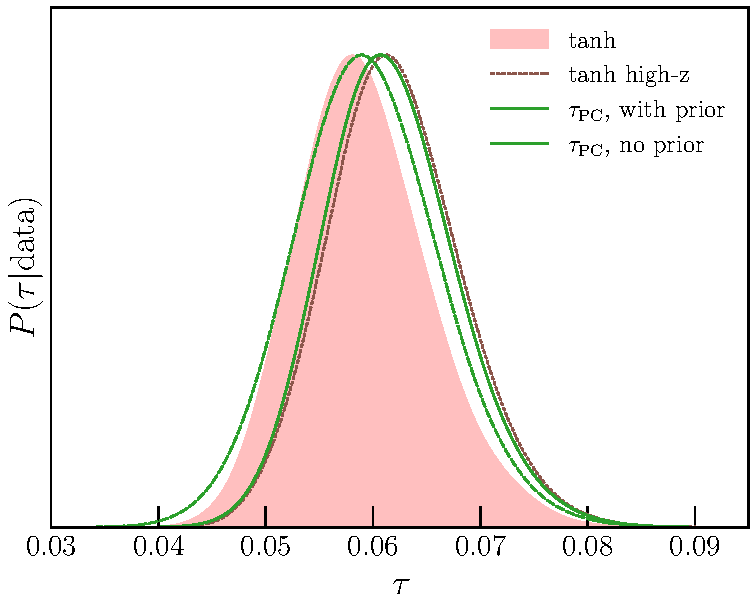
\includegraphics[width=0.48\textwidth]{results/tau_posterior_comparisons/pl18_tau_posterior_tanh_vs_tanh_highz_vs_pc_dz_auto_zre_prior_6p1_normalized_by_max.pdf}
\caption{\ch{caption to be added, will take away without prior line}}
\label{fig:tau_posterior_PC_vs_tanh_vs_tanh_highz}
\end{figure}

\begin{figure}[ht]
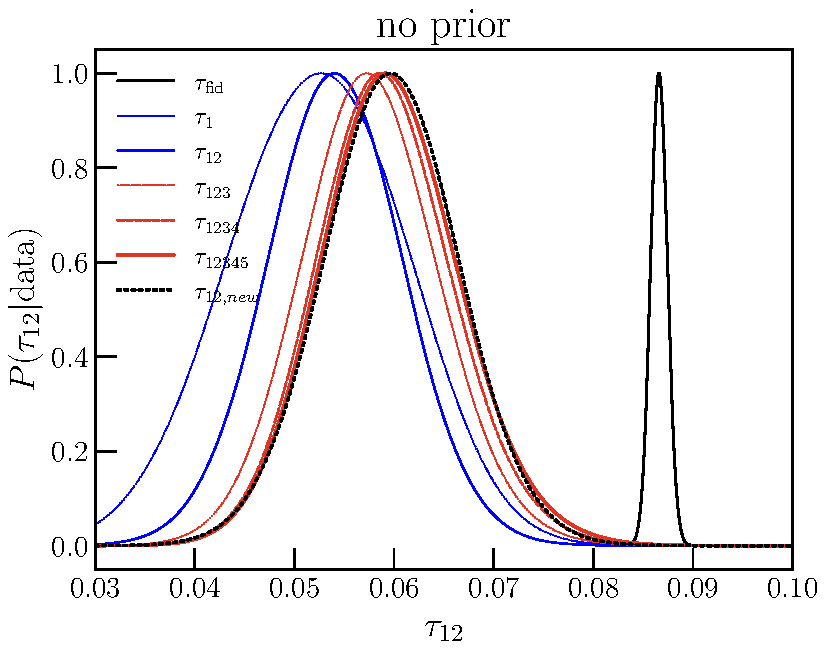
\includegraphics[width=0.48\textwidth]{results/tau_pc_decomposition/plot_taumj_decomposition_apply_cut_False_pl18_pc_zmax30_pliklite_srollv2_1015.pdf}
\caption{$\tau_{12,new}$ - this is an internal plot - leave in for now but also make a version for the paper: just $\tau_{12}$ vs $\tau_{\rm PC}$ in our new convention with and without prior either as a single or separate panel whichever is clearer.}
%\label{fig:tau12}
\end{figure}

\begin{figure}[ht]
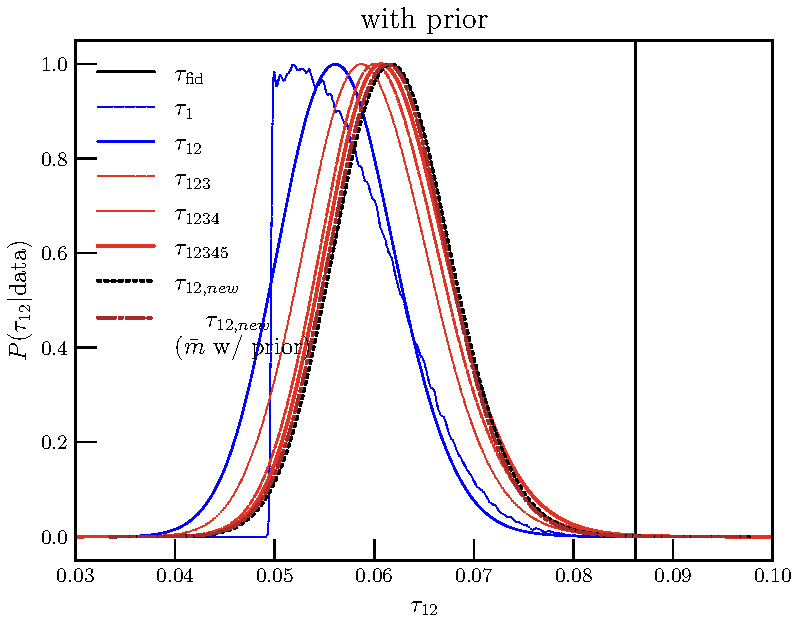
\includegraphics[width=0.48\textwidth]{results/tau_pc_decomposition/plot_taumj_decomposition_apply_cut_True_pl18_pc_zmax30_pliklite_srollv2_1015.pdf}
\caption{this is the same as above but with priors; also tested that $\tau_{12, new}$ with mean of m3, m4, m5 computed from chains with prior applied performs better here (as expected) from chains without prior.}
%\label{fig:tau12}
\end{figure}



\begin{figure}[ht]
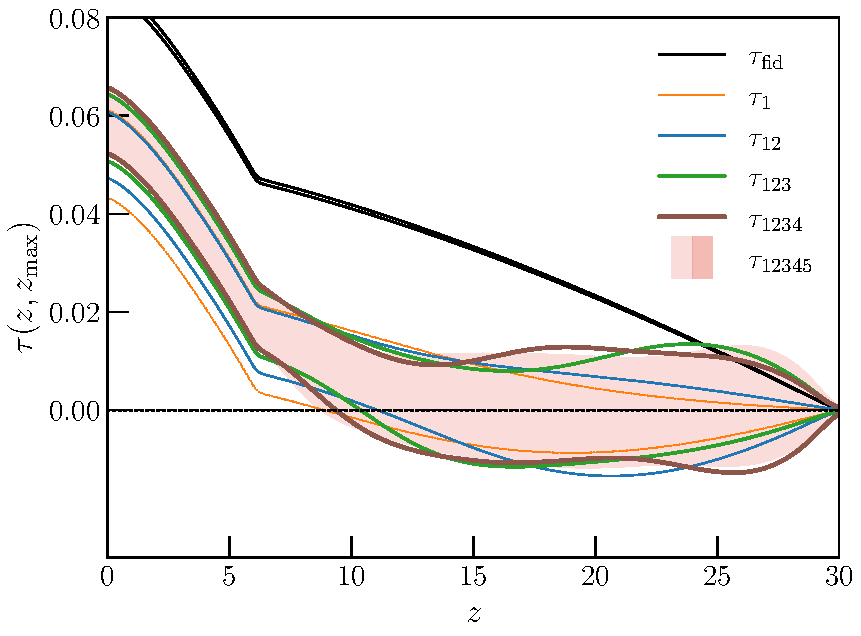
\includegraphics[width=0.48\textwidth]{results/tau_pc_decomposition/pl18_taugtz_pc_decomposition_68_only.pdf}
\caption{$\tau$ decomposition (68\% C.L. only) \wh{this is a temporary plot for internal purposes - what I'm seeing here is that without the physicality cut the high $z$ side goes unphysically negative.  I think this is consistent with our description and the $S_1$ curve.}}
%\label{fig:tau12}
\end{figure}

\begin{figure}[ht]
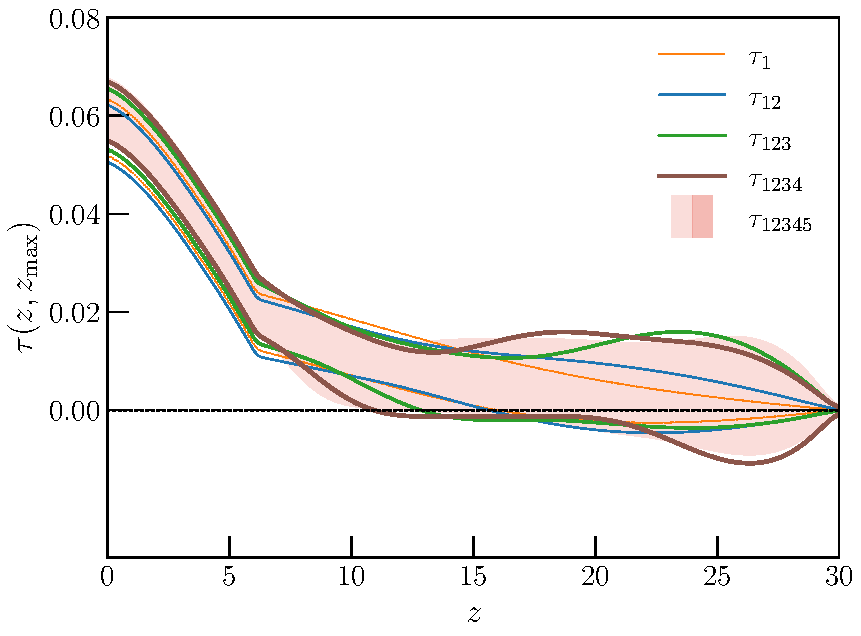
\includegraphics[width=0.48\textwidth]{results/tau_pc_decomposition/pl18_taugtz_pc_decomposition_68_only_apply_cut_True.pdf}
\caption{\ch{Internal for now (with prior version)}}
%\label{fig:tau12}
\end{figure}


\begin{table}[b]
\centering
\caption{$\tau_a$}
%\label{tab:PC_stats}
%\begin{tabular}{|r | r r r r r r|}
\begin{tabular}{|c | c | c | c | c | c|}
\hline
$\tau_{\rm fid}$ & $\tau_1$  & $\tau_2$ & $\tau_3$ & $\tau_4$ & $\tau_5$ \\ \hline
0.08626 & 0.29403 & $-$0.11227 & 0.04506 & $-$0.01898 & 0.00960 \\
\hline
\end{tabular}
\end{table}



\begin{table}[b]
\centering
\caption{PC chain means $\bar m_a$, standard deviations $\sigma(m_a)$, and correlation matrix $R_{ab}$.}
%\label{tab:PC_stats}
\begin{tabular}{|r | r r@{\hskip 0.06in}|r r r r r|}
\hline
		
			  &  \multicolumn{1}{c}{$\bar m_a$} & \multicolumn{1}{c}{$\sigma(m_a)$}	 & \multicolumn{1}{|c}{$m_1$} & \multicolumn{1}{c}{$m_2$} & \multicolumn{1}{c}{$m_3$} & \multicolumn{1}{c}{$m_4$} & \multicolumn{1}{c|}{$m_5$} 
		\\ \hline
		

$m_1$ & $-$0.116 & 0.030 & 1.000 & 0.657 & $-$0.208 & $-$0.094 & 0.067 \\
$m_2$ & $-$0.016 & 0.063 & 0.657 & 1.000 & 0.048 & $-$0.273 & 0.142 \\
$m_3$ & $$0.078 & 0.098 & $-$0.208 & 0.048 & 1.000 & 0.064 & $-$ \\
$m_4$ & $-$0.077 & 0.131 & $-$0.094 & $-$0.273 & 0.064 & 1.000 & $-$0.195 \\
$m_5$ & 0.066 & 0.145 & 0.067 & 0.142 & $-$0.018 & $-$0.195 & 1.000 \\

\hline
\end{tabular}
\end{table}

% all digits without flipping m3, m4:
%tau_fid 0.08625526676478058
%taumj [ 0.29403315 -0.11227135 -0.04505736  0.0189787   0.00960184
\begin{table}[b]
\centering
\caption{Planck 2015 results (with Mortonson PCs) [Will not be in the paper, just for us to compare] }
%\label{tab:PC_stats}
\begin{tabular}{|r | r r@{\hskip 0.06in}|r r r r r|}
\hline
		
			  &  \multicolumn{1}{c}{$\bar m_a$} & \multicolumn{1}{c}{$\sigma(m_a)$}	 & \multicolumn{1}{|c}{$m_1$} & \multicolumn{1}{c}{$m_2$} & \multicolumn{1}{c}{$m_3$} & \multicolumn{1}{c}{$m_4$} & \multicolumn{1}{c|}{$m_5$} 
		\\ \hline

$m_1$ 
	& 0.002 & 0.053 & 1.000 & 0.450 & $-$0.432 & 0.273 & $-$0.073 \\ 
$m_2$ 
	& $-$0.030 &  0.101 & 0.450 & 1.000 & $-$0.262 & 0.055 & 0.072 \\ 
$m_3$ 
	& 0.019 &  0.128 & $-$0.432 & $-$0.262 &1.000 & $-$0.417 & 0.155 \\
$m_4$  
	& $-$0.012 & 0.143 &  0.273 & 0.055 & $-$0.417 & 1.000 & $-$0.428 \\ 
$m_5$ 
	& 0.026 & 0.143 & $-$0.073 & 0.072 & 0.155 & $-$0.428 & 1.000\\ 
\hline
\end{tabular}
\end{table}

% Notes:
% tau1 = (taulo + tauhi) --> (zre, xemin) --> xe(z) ==> tau2 ==> mjs --> tau3(mjs)
% taulo + tauhi = tau_desired 

\begin{figure}
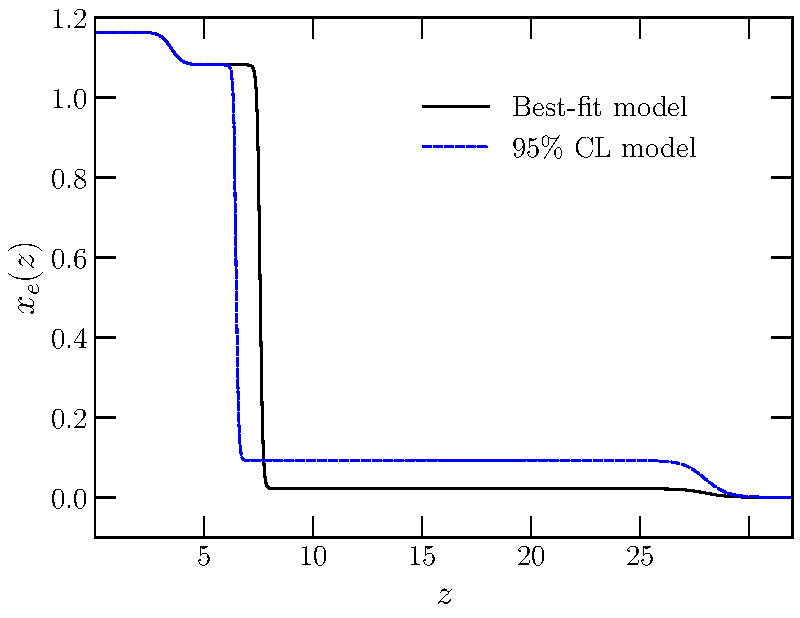
\includegraphics[width=0.48\textwidth]{paper/plots/plot_xe_tanh_highz.pdf}
\caption{Two step ionization history $x_e(z)$ for the model of \refsec{example2}. In addition to a tanh transition at low-redshift as in \refsec{example1}, there is an additional ionization plateau at high redshifts with a fixed transition at $z_t = 28$ and $\Delta z = 1$. Here we show the best-fit model in the Planck 2018 data $(\taulo, \tauhi) = (0.053, 0.006)$, as well as  a model on the 95\% C.L. contour of Fig.~\ref{fig:two_parameter_model_2D}, $(\taulo, \tauhi) = (0.043, 0.026)$. 
%best-fit (0.05290344, 0.005859431)
%95\%CL (0.0427, 0.0256): zre = 6.4685, xemin = 0.0925 
}
\label{fig:two_step_model}
\end{figure}

\end{document}



%\ch{Should we do a table giving an overview of tau measurement evolution from Planck collaboration and in the literature, for tanh and other model-independent approaches?}
%\todo{e.g.
%Planck 2015 (LFI only)\\
%Planck 2016 XLVI(\cite{Aghanim:2016yuo}) with reduction of systematics for HFI \\
%Planck 2016 XLVII (\cite{Adam:2016hgk}) - intermediate results LFI + HFI, tanh\\
%Ref.~\cite{Millea:2018bko} - intermediate results LFI + HFI generic model. \\
%Planck 2018 cosmological parameters paper LFI + HFI w/ SimAll low-l EE likelihood (FlexKnot)\\
%Srollv2 measurement Ref.~\cite{Pagano:2019tci}
%}
%